%%% Hlavní soubor. Zde se definují základní parametry a odkazuje se na ostatní části. %%%

%% Verze pro jednostranný tisk:
% Okraje: levý 40mm, pravý 25mm, horní a dolní 25mm
% (ale pozor, LaTeX si sám přidává 1in)
\documentclass[12pt,a4paper]{report}
\setlength\textwidth{145mm}
\setlength\textheight{247mm}
\setlength\oddsidemargin{15mm}
\setlength\evensidemargin{15mm}
\setlength\topmargin{0mm}
\setlength\headsep{0mm}
\setlength\headheight{0mm}
% \openright zařídí, aby následující text začínal na pravé straně knihy
\let\openright=\clearpage

%% Pokud tiskneme oboustranně:
% \documentclass[12pt,a4paper,twoside,openright]{report}
% \setlength\textwidth{145mm}
% \setlength\textheight{247mm}
% \setlength\oddsidemargin{15mm}
% \setlength\evensidemargin{0mm}
% \setlength\topmargin{0mm}
% \setlength\headsep{0mm}
% \setlength\headheight{0mm}
% \let\openright=\cleardoublepage

%% Pokud používáte csLaTeX (doporučeno):
\usepackage{czech}
%% Pokud nikoliv:
%\usepackage[czech]{babel}
%\usepackage[T1]{fontenc}

%% Použité kódování znaků: obvykle latin2, cp1250 nebo utf8:
%\usepackage[latin2]{inputenc}
\usepackage[utf8]{inputenc}

%% Ostatní balíčky
\usepackage{graphicx}
\usepackage{amsthm}

%% Balíček hyperref, kterým jdou vyrábět klikací odkazy v PDF,
%% ale hlavně ho používáme k uložení metadat do PDF (včetně obsahu).
%% POZOR, nezapomeňte vyplnit jméno práce a autora.
\usepackage[ps2pdf,unicode]{hyperref}   % Musí být za všemi ostatními balíčky
\hypersetup{pdftitle=AJAX CAT - webový editor s podporou pro překlad}
\hypersetup{pdfauthor=Ondřej Odcházel}

%%% Drobné úpravy stylu

% Tato makra přesvědčují mírně ošklivým trikem LaTeX, aby hlavičky kapitol
% sázel příčetněji a nevynechával nad nimi spoustu místa. Směle ignorujte.
\makeatletter
\def\@makechapterhead#1{
  {\parindent \z@ \raggedright \normalfont
   \Huge\bfseries \thechapter. #1
   \par\nobreak
   \vskip 20\p@
}}
\def\@makeschapterhead#1{
  {\parindent \z@ \raggedright \normalfont
   \Huge\bfseries #1
   \par\nobreak
   \vskip 20\p@
}}
\makeatother

% Toto makro definuje kapitolu, která není očíslovaná, ale je uvedena v obsahu.
\def\chapwithtoc#1{
\chapter*{#1}
\addcontentsline{toc}{chapter}{#1}
}

\begin{document}

% Trochu volnější nastavení dělení slov, než je default.
\lefthyphenmin=2
\righthyphenmin=2

%%% Titulní strana práce

\pagestyle{empty}
\begin{center}

\large

Univerzita Karlova v Praze

\medskip

Matematicko-fyzikální fakulta

\vfill

{\bf\Large BAKALÁŘSKÁ PRÁCE}

\vfill

\centerline{\mbox{
\includegraphics[width=60mm]{logo.eps}}}

\vfill
\vspace{5mm}

{\LARGE Ondřej Odcházel}

\vspace{15mm}

% Název práce přesně podle zadání
{\LARGE\bfseries AJAX CAT - webový editor s podporou pro překlad}

\vfill

% Název katedry nebo ústavu, kde byla práce oficiálně zadána
% (dle Organizační struktury MFF UK)
Ústav formální a aplikované lingvistiky

\vfill

\begin{tabular}{rl}

Vedoucí diplomové práce: & RNDr. Ondřej Bojar, Ph.D. \\
\noalign{\vspace{2mm}}
Studijní program: & Informatika \\
\noalign{\vspace{2mm}}
Studijní obor: & Programování \\
\end{tabular}

\vfill

% Zde doplňte rok
Praha 2011

\end{center}

\newpage

%%% Následuje vevázaný list -- kopie podepsaného "Zadání diplomové práce".
%%% Toto zadání NENÍ součástí elektronické verze práce, nescanovat.

%%% Na tomto místě mohou být napsána případná poděkování (vedoucímu práce,
%%% konzultantovi, tomu, kdo zapůjčil software, literaturu apod.)

\openright

\noindent
Poděkování.

\newpage

%%% Strana s čestným prohlášením k diplomové práci

\vglue 0pt plus 1fill

\noindent
Prohlašuji, že jsem tuto diplomovou práci vypracoval samostatně a výhradně
s~použitím citovaných pramenů, literatury a dalších odborných zdrojů.

\medskip\noindent
Beru na~vědomí, že se na moji práci vztahují práva a povinnosti vyplývající
ze zákona č. 121/2000 Sb., autorského zákona v~platném znění, zejména skutečnost,
že Univerzita Karlova v Praze má právo na~uzavření licenční smlouvy o~užití této
práce jako školního díla podle §60 odst. 1 autorského zákona.

\vspace{10mm}

\hbox{\hbox to 0.5\hsize{%
V ........ dne ............
\hss}\hbox to 0.5\hsize{%
Podpis autora
\hss}}

\vspace{20mm}
\newpage

%%% Povinná informační strana diplomové práce

\vbox to 0.5\vsize{
\setlength\parindent{0mm}
\setlength\parskip{5mm}

Název práce:
AJAX CAT - webový editor s podporou pro překlad
% přesně dle zadání

Autor:
Ondřej Odcházel

Katedra:  % Případně Ústav:
Ústav formální a aplikované lingvistiky
% dle Organizační struktury MFF UK

Vedoucí diplomové práce:
RNDr. Ondřej Bojar, Ph.D., Ústav formální a aplikované lingvistiky
% dle Organizační struktury MFF UK, případně plný název pracoviště mimo MFF UK

Abstrakt:
% abstrakt v rozsahu 80-200 slov; nejedná se však o opis zadání diplomové práce

Klíčová slova:
% 3 až 5 klíčových slov

\vss}\nobreak\vbox to 0.49\vsize{
\setlength\parindent{0mm}
\setlength\parskip{5mm}

Title:
% přesný překlad názvu práce v angličtině

Author:
Jméno a příjmení autora

Department:
Název katedry či ústavu, kde byla práce oficiálně zadána
% dle Organizační struktury MFF UK v angličtině

Supervisor:
Jméno a příjmení s tituly, pracoviště
% dle Organizační struktury MFF UK, případně plný název pracoviště
% mimo MFF UK v angličtině

Abstract:
% abstrakt v rozsahu 80-200 slov v angličtině; nejedná se však o překlad
% zadání diplomové práce

Keywords:
% 3 až 5 klíčových slov v angličtině

\vss}

\newpage

%%% Strana s automaticky generovaným obsahem diplomové práce. U matematických
%%% prací je přípustné, aby seznam tabulek a zkratek, existují-li, byl umístěn
%%% na začátku práce, místo na jejím konci.

\openright
\pagestyle{plain}
\setcounter{page}{1}
\tableofcontents

%%% Jednotlivé kapitoly práce jsou pro přehlednost uloženy v samostatných souborech
\chapter*{Úvod}
\addcontentsline{toc}{chapter}{Úvod}

Díky novým statistickým přístupům zažívá obor strojového překladu jazyka v posledních letech opět velký rozvoj. Nové výpočetní i algoritmické možnosti umožňují vytváření stále lepších jazykových překladů. Stále se však nepodařilo vytvořit univerzální překladový systém, který by dokázal nahradit lidské překladatele, ani v jednom běžném jazykovém páru. Je stále otázka zdali se podobný překladový systém v budoucnosti lidstvu podaří sestavit. Již dnes jsou ale překladové systémy na úrovni, která sice nedokáže překladatele nahradit, ale v mnoha odvětvích usnadňuje jejich práci. Překladové systémy již nyní poskytují alespoň nápovědu, jak daný text přeložit. Překladatel však stále musí výstup z takového systému kontrolovat a editovat. Každý z těchto editačních zásahů představuje pro překladatele komplikaci a pokud je množství nutných zásahů nad nějakou hranicí, překladatel raději místo editování výstupu překladového systému vytvoří překlad sám. Pro zjednodušení překladatelské práce je tedy potřeba nejen zlepšovat tyto překladové systémy, ale také software kteří překladatelé pro interakci s překladovým systémem používají. Překladový software, který využívá pro nápovědu překladatelům strojový překlad je speciální případem CAT (computer--aided translation) systému.

Cílem této bakalářské práce je implementace jednoho CAT systému. Pro podporu překladu bude systém využívat překladový systém Moses. Celý projekt je rozdělen do dvou částí --- serverová a klientská část. Implementací serverové části bude vytvořen HTTP server. Tento server bude spouštět Mosese a skrz HTTP požadavky bude poskytovat klientovi odpovědi. Požadavky budou dvojího typu. Klient se může systému zeptat na překlad věty v určité jazyce. Server pak odpoví tabulkou překladových možností. Sloupce této tabulky jsou jednotlivé úseky ve zdrojovém překladovém úseku (typicky slova ve větě). V řádcích tabulky jsou pak přeložené úseky textu v cílovém jazyce. Úseky jsou seřazeny v tabulce tak, že čím výše je daný úsek, tím větší je pravděpodobnost toho, že se jedná o "správný překlad". Taková to tabulka je jedním ze základů implementovaného CAT systému.

Dalším typem klientského požadavku bude jakási lokální nápověda během překladu. Jedná se o podobný druh nápovědy jakou nám poskytují například intenetové vyhledávače. V nich často uživatel nemusí psát celý vyhledávací dotaz a může využí nápovědy, která mu nabízí nejběžnější podobné dotazy. Podobně i implementovaný server bude dávat nápovědu, jak dále pokračovat s překladem. Aby překladový systém mohl tuto nápovědu poskytnout, pořebuje znát tři parametry. Text ve zdrojovém jazyce, vektor určující, které úseky jsou již přeloženy a již přeložená část věty v cílovém jazyce. Cílem této práce je i rozšířit možnosti Mosese tak, aby s těmito třemi parametry dokázal pracovat a vygeneroval nápovědu, jak v překladu pokračovat.

Samotná serverová část tak bude moci fungovat jako komponenta samostatně a poskytovat nápovědu k překladu i jiném CAT systému.

Druhou částí práce je implementace klientské části CAT systému. Tato část bude sloužit k interakci překladatele s překladový systémem. Tato interakce by měla být co nejvíce přátelská k uživateli. Ten typicky zadá zdrojový text pro překlad a zdrojový a cílový jazyk překladu. CAT systém tento zdrojový text rozseká do bloků (typicky vět) a ke každé větě překladateli nabídne nápovědu generovanou v serverové části. Součástí implementace klientské části bude i jednoduchý systém pro zprávu obsahu, aby překladatel mohl pokračovat v překladu i po znovuotevření aplikace. Klientská část bude podobně jako serverová část fungovat sama o sobě. Pokud tedy nebude napojena na server, může pracovat sama o sobě jako systém pro správu překladů.




\chapter{Překlad a strojový překlad}

\section{Překladové problémy}

Překlad je proces přenesení významu z textu ve zdrojovém jazyce do jazyka cílového. Úloha překladu je složitá i tím, že žádný výsledek nejde označit za nejlepší. Že neexistuje dokonalý překlad lze ilustrovat na překladech knih, nebo divadelních her. Hry Williama Shakespearea byly z angličtiny do češtiny přeloženy mnohokrát, přesto jsou stále inscenovány hry s různými překlady.

Bez hlubších jazykových znalostí se může jevit úloha překladu snadná, mezi většinou jazyků máme přeci slovník. Ale pokud chceme přeložit anglické slovo "house" do češtiny, můžeme mít problém. Ve většině případů lze toto slovo přeložit jako "dům". Pokud ale překládáme text o anglické královně, kde se objeví sousloví "House of Windsor", zřejmě není řeč o domu, kde bydlí Windsorové, ale o "rodu Windsorů". Překladatel tedy při textu potřebuje znát kontext ve kterém je slovo použito a často také potřebuje mít odborné znalosti z oboru překládaného textu.

Jazyk není neměnný a v průběhu času se vyvíjí. Můžeme to vidět například na Bibli. Její nejznámější překlad, Bible Kralická je přes 300 (?) let starý. Vznikají proto nové překlady, které jsou dnešním čtenářům přístupnější. Žádný překlad tedy nelze označit za dokonalý a navždy správný.

\section{Historie strojového překladu}

Na počátku dějin strojového překladu stála, podobně jako v mnoha jiných oborech, armáda. Spojené státy Americké byli v padesátých letech ve Studené válce se Sovětským svazem. V této válce beze zbraní sehráli velkou úlohu i výzvědné služby, které zachytávali velké množství nepřátelských zpráv. Tyto zprávy bylo nutné co nejrychleji přeložit. A právě v této době se zrodila myšlenka použít k tomuto účelu počítače, které byli produktem předchozího válečného konfliktu, 2. světové války. ( http://www.hutchinsweb.me.uk/GU-IBM-2005.pdf ) Významnou demonstrací použití strojového překladu se v roce 1954 stal takzvaný Georgetownský experiment. Pro tento experiment vyvinula Georgetownská univerzita spolu s firmou IBM překladový systém pro překlad z ruštiny do angličtiny. Tento systém používal slovník 250 slov a 6 gramatických pravidel. Jeho doménou byly zejména překlady v oblasti chemie. Během experimentu bylo přeloženo více než 60 vět. Experiment byl všeobecně přijat jako úspěch, což donutilo americkou vládu investovat v následujících letech do oblasti strojového překladu.

Následovaly léta práce zejména v SSSR a USA na systémech pro automatické překlady zejména mezi ruštinou a angličtinou. Žádný dobře použitelný systém, který by poskytoval uspokojivé výsledky, však nevzniknul. Pochybnosti ohledně možností strojového překladu vyjádřil na konci padesátých let lingvista Yehoshua Bar-Hillel. Ten argumentoval pomocí anglické věty "The box was in the pen." Překlad této věty by mohl být: "Pero bylo v ohradě." Jelikož anglické slovo "pen" znamená "pero" i "ohrada", musí mít překladový systém, který chce větu přeložit správně, sémantickou informaci, která by mu napověděla, že krabice nemůže být peru, tedy že správným překladem slova "pen" do češtiny je v tomto kontextu slovo "ohrada".

http://www.hutchinsweb.me.uk/ALPAC-1996.pdf
I z tohoto důvodu bylo vytvoření komplexního překladového systému v té době zřejmě nemožné. Americká vláda však dále pokračuje ve financování výzkumu. V roce 1966 vyšla zpráva skupiny ALPAC (Automatic Language Processing Advisory Committee). Která doporučovala americké vládě další postup při financování překladového výzkumu. Zpráva zmenšovala optimismus, vyvolaný zejména Georgetownským experimentem, že se v dohledné době podaří vytvořit kvalitní systém pro strojový překlad. Výsledkem bylo téměř úplné zastavení financování výzkumu americkou vládou. Výzkum dále pokračoval zejména v Evropě, nebo Kanadě. Právě v kanadském Montrealu vznikl systém METEO. Ten byl v letech 1981 až 2001 používán pro překlad meteorologických zpráv mezi angličtinou a francouzštinou. Právě omezená překladová doména systému umožnila nabízet kvalitní překlady předpovědí počasí.


\section{Součastnost strojového překladu}
V posledních letech spolu s pokračující globalizací světa a stále vyšší penetrací internetového připojení se zvyšuje i poptávka po překladech. Nadnárodní firmy potřebují při svém růstu stále více překladů. Dalším impulzem zvyšujícím popávku po překladech je i rozšiřování Evropské Unie. V součastnosti unie používá 23 oficiálních jazyků ve kterých musí být přístupné všechny důležité úřední dokumenty. Tvorba tolika překladů je velice pracná a nákladná, což vytváří poptávku po zjednodušením procesu překladu.

Výpočetní výkon počítačů stále roste rychlostí Mooreova zákona (ftp://download.intel.com/research/silicon/moorespaper.pdf), což v posledních letech otevřelo možnosti pro použití statistických metod ve strojovém překladu. Toho využívá statistický překladový systém Moses, open-source překladový systém, který používám i ve svém projektu a cílem projektu byla i implementace nových rozšíření. Dalším známým statistickým překladovým systémem je Google Translate.

Kromě systému využívajících statických postupů se stále vyvíjí i pravidlové překladové systémy. Kromě mnoha proprietálních systémů bych zmínil open-source systém Apertium. Stejně jako u dalších podobných systémů se pro každou dvojici překládaných jazyků musí vytvořit slovníky a překladová pravidla. Je velmi náročné a nákladné tato pravidla vytvořit. Navíc jsou tato pravidla často použitelná pouze pro jeden jazykový pár.

\section{Computer-aided translation}
CAT, neboli computer-aided translation, či computer-assisted translation je zkratka označující systémy pro podporu překladu. Tyto systémy poskytují překladateli podporu při překladu. Mohou to být jak desktopové, tak online aplikace a často se liší stylem, jakým překladatele podporují. Jedním z druhů podpory může být nabídka předchozích překladů z paměti. Této paměti se říká překladová paměť, obsahuje přeložené úseky textu a překladatel si tuto paměť buduje buď sám, nebo může využít nějakou z kolektivních databází. Příkladem desktopové aplikace může být například OmegaT. Ta je určena pro použití profesionálními překladateli, kterým nabízí úseky z překladové paměti. Hledaný úsek nemusí odpovídat aktuálně překládanému úseku na 100 procent, OmegaT implementuje algoritmus, který pozná i blízké shody.

Další ukázkou CAT pomůcky je Google Translator Toolkit (Nástroje pro překladatele). Tato internetová aplikace umožňuje překladateli nahrát si svou překladovou paměť, kterou pak může využít při překladu. Dále nástroj nabízí výsledky překladu z Google Translate, který dále může uživatel editovat.

\section{Moses}


\chapter{Moses}

Moses je statistický překladový systém založený na překladu frází (anglicky PBMT - phrase-based machine translation). 

\section{Princip frázového překladu}

\begin{figure}[ht]
\begin{center}
\includegraphics[scale=0.5,bb=36 36 416 186]{pictures/phrase-based.eps}
\end{center}
\caption{Architektura frázových překladových systémů.}
\label{phrase-based-models}
\end{figure}

Součastné nejvyspělejší generické (tedy více či méně nezávislé na jazykovém páru) překladové systémy jsou založeny na překladu frází. Jejich architektura je znázorněna na Obrázku \ref{phrase-based-models}.

\section{Jazykový a překladový model}
Tyto systémy používají k překladu vstupu na výstup překladový a jazykový model. Překladový model zachycuje četnost překladů frází délky n. Tyto fráze jsou také označovany jako n-gramy. Překladový model lze získat z paralelních korpusů, tedy přeložených textů mezi zdrojovým a cílovým jazykem. Jazykový model zachycuje četnost výskytu frází v cílovém jazyce. Pro jeho získání tedy stačí texty v cílovém jazyce. Díky překladovému a jazykovému modelu lze získat různé překlady frází ve vstupním textu. Pro vygenerování výstupu potřebuje překladový systém nalézt posloupnost frází v cílovém jazyce, které pokrývají všechny části vstupu a mají největší pravděpodobnost výskytu.

\section{Hledání nejlepších hypotéz}
Při generování překladu používá Moses strukturu, která se anglicky nazývá "lattice", neboli graf slov.

Variant překladu může být obecně exponenciální množství. Pro rychlé hledání v těchto variantách implementuje Moses tzv. beam search algoritmus. Postup algoritmu při hledání zobrazuje Obrázek 2.2. Jedná se vlastně o orientovaný graf. Vrcholy grafu znázorňují částečné hypotézy. Každá taková částečná hypotéza pokrývá nějaká slova ze vstupu a má skóre, které určuje kvalitu hypotézy. Na začátku je překladu je prázdná hypotéza, která nepokrývá žádnou část vstupu. Na konci máme hypotézy které pokrývají celý vstup. Během překladu překladový systém postupně rozšiřuje exitující hypotézy o další fráze. Hypotéza s nejvyšším skóre je nabídnuta jako překlad na výstup. Pomocí tabulky překladovýchmožností dokáže Moses poskytnou i další hypotézy seřazené podle pravděpodobnosti.

\section{Rozšíření Mosese}
Pro poskytnutí nápovědy během překladu bylo nutné rozšířit možnosti Mosese tak, aby dokázal generovat hypotézy z neprázdné počáteční hypotézy. Překladatel je uprostřed překladu věty, má přeložená určitá slova a potřebuje radu, jak nejlépe pokračovat dál. Pomocí implementovaného rozšíření se nyní může zeptat Mosese, který může začít generovat překlad navazující na již přeloženou část. K tomu potřebuje vektor označující části vstupní věty, které byly již přeloženy. Kvůli jazykovému modelu, který kontroluje, aby navazující část byla v cílovém jazyce co nejvíce smysluplná, potřebuje Moses znát část přeloženého textu, na kterou se může pokusit navázat. Pomocí tohoto rozšíření může Moses začít rozvíjet hypotézy, které se v prvotním překladu z prázdné hypotézy nemusely vůbec objevit. Toto by mělo přispět k flexibilitě nápovědy. Správný překlad totiž leckdy může být specifický a použitá slova nemusí být v překladovém modelu vůbec použita.










\chapter{Implementace}

\section{Instalace serverové části}

\section{Instalace klientské části}

\include{kap4}

% Ukázka použití některých konstrukcí LateXu (odkomentujte, chcete-li)
% %%% Ukázka použití některých konstrukcí LaTeXu

\subsection{Ukázka \LaTeX{}u}
\label{ssec:ukazka}

V~této krátké části ukážeme použití několika základních konstrukcí \LaTeX{}u,
které by se vám mohly při psaní práce hodit.

Třeba odrážky:

\begin{itemize}
\item Logo Matfyzu vidíme na obrázku~\ref{fig:mff}.
\item Tato subsekce má číslo~\ref{ssec:ukazka}.
\item Odkaz na literaturu~\cite{lamport94}.
\end{itemize}

Druhy pomlček:
červeno-černý (krátká),
strana 16--22 (střední),
$45-44$ (minus),
a~toto je --- jak se asi dalo čekat --- vložená věta ohraničená dlouhými pomlčkami.
(Všimněte si, že jsme za \verb|a| napsali vlnovku místo mezery: to aby se
tam nemohl rozdělit řádek.)

% Makro na české uvozovky (novější verze LaTeXu ho už mají zabudované)
\newcommand{\uv}[1]{\quotedblbase #1\textquotedblleft}
\uv{České uvozovky.}

\newtheorem{theorem}{Věta}
\newtheorem*{define}{Definice}	% Definice nečíslujeme, proto "*"

\begin{define}
{\sl Strom} je souvislý graf bez kružnic.
\end{define}

\begin{theorem}
Tato věta neplatí.
\end{theorem}

\begin{proof}
Neplatné věty nemají důkaz.
\end{proof}

\begin{figure}
	\centering
	
\includegraphics[width=30mm]{logo.eps}
	\caption{Logo MFF UK}
	\label{fig:mff}
\end{figure}


\chapter*{Závěr}
\addcontentsline{toc}{chapter}{Závěr}


%%% Seznam použité literatury
%%% Seznam použité literatury je zpracován podle platných standardů. Povinnou citační
%%% normou pro diplomovou práci je ISO 690. Jména časopisů lze uvádět zkráceně, ale jen
%%% v kodifikované podobě. Všechny použité zdroje a prameny musí být řádně citovány.

\def\bibname{Seznam použité literatury}
\begin{thebibliography}{99}
\addcontentsline{toc}{chapter}{\bibname}

\bibitem{lamport94}
  {\sc Lamport,} Leslie.
  \emph{\LaTeX: A Document Preparation System}.
  2. vydání.
  Massachusetts: Addison Wesley, 1994.
  ISBN 0-201-52983-1.

\end{thebibliography}


%%% Tabulky v diplomové práci, existují-li.
\chapwithtoc{Seznam tabulek}

%%% Použité zkratky v diplomové práci, existují-li, včetně jejich vysvětlení.
\chapwithtoc{Seznam použitých zkratek}

%%% Přílohy k diplomové práci, existují-li (různé dodatky jako výpisy programů,
%%% diagramy apod.). Každá příloha musí být alespoň jednou odkazována z vlastního
%%% textu práce. Přílohy se číslují.
\chapwithtoc{Přílohy}

\openright
\end{document}
